\subsection{Outline of the Theory on DevOps Adoption}

We summarize our theory in this section using a 
set of recommendations about building and reporting
theories in software engineering~\cite{sjoberg2008}.
Accordingly, a theory should be described in
terms of {\bf constructs},
{\bf propositions}, {\bf explanation} for the propositions,
and {\bf scope} of the theory.

The main construct of our theory is \emph{DevOps adoption},
which means any effort for building a \cc between
the development and operations teams. DevOps adoption is
supported by other constructs, including \emph{automation}
(deployment automation, infrastructure provision automation,
test automation, and so on) and knowledge sharing (e.g.,
sharing procedures and making clear the task assignments
of the teams). We augmented our hypothesis to identify
a set of nine propositions, which we can explain
by means of the categories, categories' relations,
and transcription memos. For instance, the necessity of
using tech talks, simplifying communication procedures, and employing
tools like Slack and Hip Chat explains the relevance of knowledge sharing
(P2). Similarly, we can explain proposition (P7) by 
considering our research transcriptions, like
``\emph{DevOps reduces (or even eliminates) downtime}''.
The scope of our theory relates to
enterprise systems (in particular those based on
a service-oriented architecture). 


\begin{enumerate}[(P1)]
 \item The use of automation enables DevOps
 \item The use of practices and tools for sharing knowledge enables DevOps
 \item The use of continuous measurement procedures enables DevOps
 \item The use of quality assurance methods enables DevOps
 \item DevOps centered on \cc increases the agility of the teams
 \item DevOps centered on \cc increases systems' resilience 
 \item DevOps centered on \cc decrease systems'  downtime
 \item DevOps centered on \cc supports continuous measurement 
 \item DevOps centered on \cc supports SQA activities   
\end{enumerate}

Figure~\ref{fig:theory} represents the elements of our theory using the
notation introduced in~\cite{sjoberg2008}. In this notation,
a construct is either represented as a class (light grey
boxes) or as an attribute of a class (white boxes within classes).
Relationships model the propositions as arrows, and the direction
of the arrow models a cause-effect relation. For instance,
in Figure~\ref{fig:theory}, the \emph{DevOps Collaborative Culture}
increases the agility of both development and operations teams
(proposition (P5).


\begin{figure}[htb]
  \centering{
    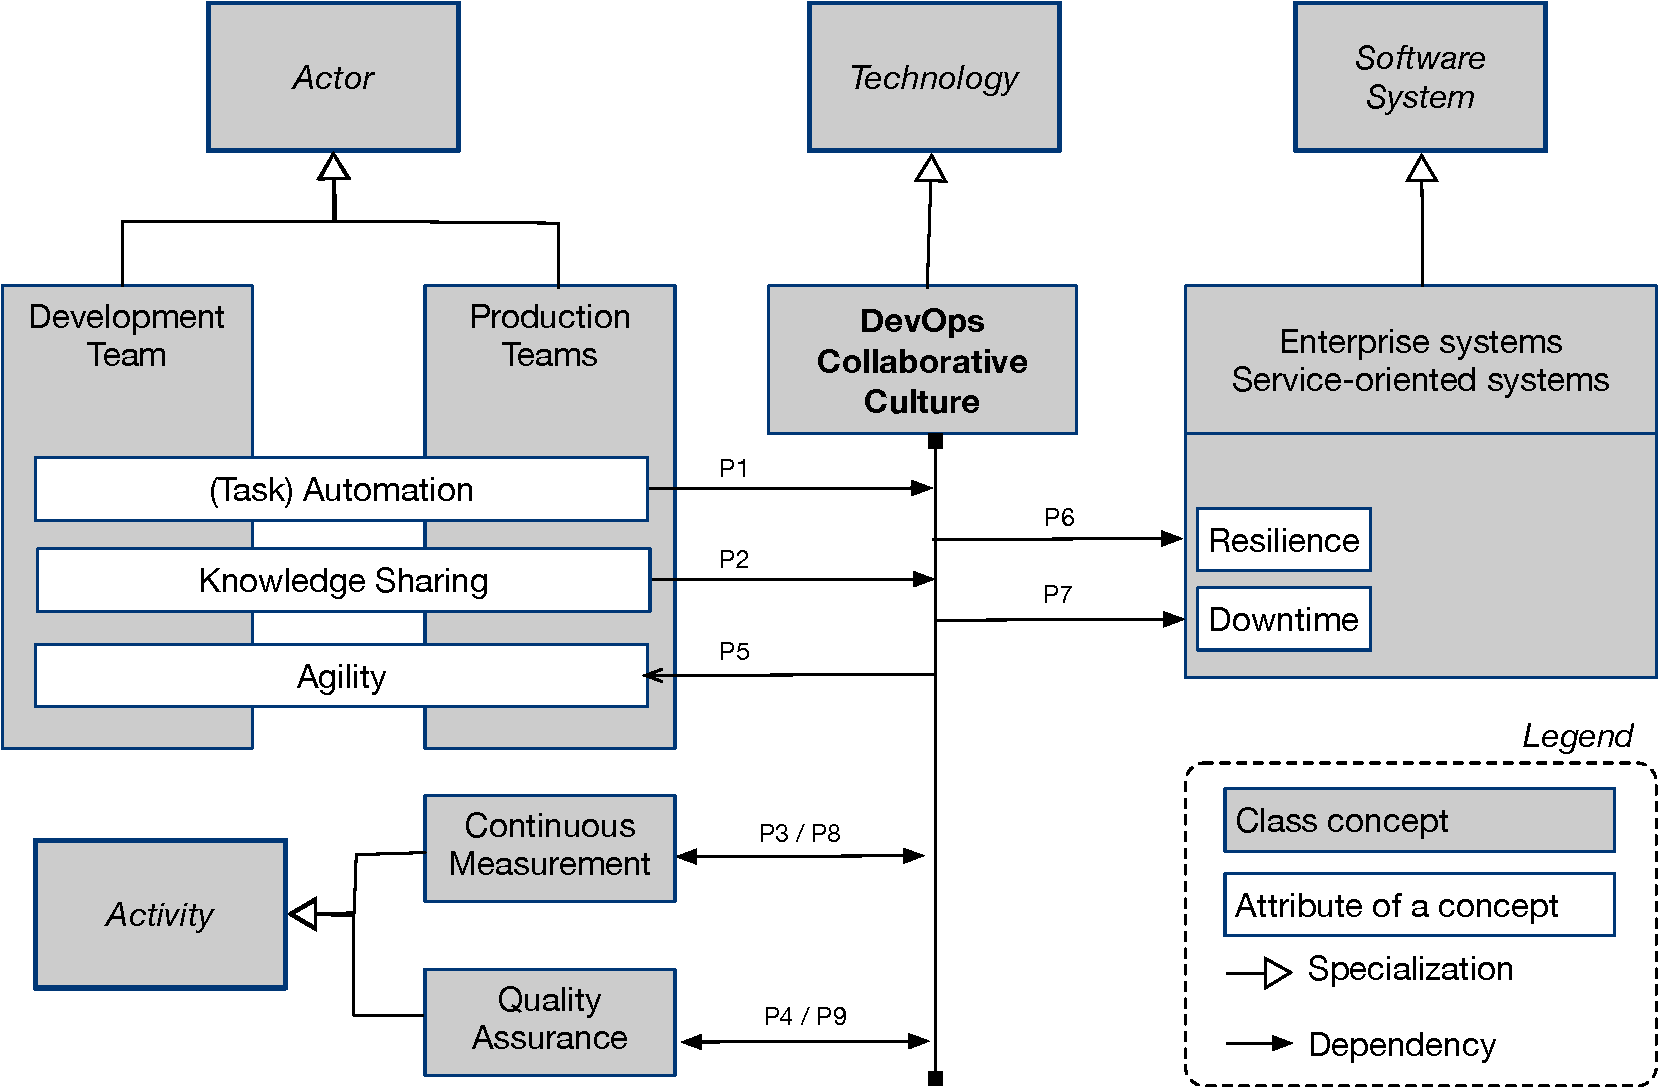
\includegraphics[width=0.8\textwidth]{images/theory.pdf}
  }
  \caption{A Theory for DevOps Adoption}
  \label{fig:theory} 
\end{figure}



